\subsubsection{Minuta de reunião (27-Janeiro-2016)}

\begin{tabbing}
  Local \= xxx \kill
  Local \> : LEAD \\
  Data  \> : 27 de Janeiro de 2016 \\
  Hora  \> : 10:00
\end{tabbing} 

%---------------------------------------------------------------------
\participantes{
  \gabriel,
  \julia,
  \estevão,
  \elael,
  \renan,
  \ramon.

}

\textbf{Aprovação da minuta}

\textbf{Update semanal do Projeto EMMA}

						
\textbf{\gabriel.} 
	\begin{itemize}
			\item Relatório de localização da pá.
			\item Implementação de verificação de hipóteses de modelos encontrados.
			\end{itemize}
		
		\item \textbf{Novas tarefas:}
			\begin{itemize} 
				\item Implementar localização da pá no framework a ser utilizado no robô.
			\end{itemize}

					
   \textbf{\estevão.} 
	\begin{itemize}
		\item \textbf{Tarefas concluídas:}
			\begin{itemize}    
			    \item Conjunto de peças do trilho.
			    \item Reunião Bosch.
			    \item Definir peças a serem compradas no Brasil.
				
			\end{itemize}
		
		\item \textbf{Novas tarefas:}
			\begin{itemize} 
			    \item Rotação e elevação da base.
			\end{itemize}
	\end{itemize}

	
	  \textbf{\elael.} 
	\begin{itemize}
		\item \textbf{Tarefas concluídas:}
			\begin{itemize}    
				\item Enviou motivação, objetivos e metodologia para o orientador.
			\end{itemize}
		
		\item \textbf{Novas tarefas:}
			\begin{itemize} 
			    \item Revisão bibliográfica do Mestrado.
			    \item Verificação de trajetória.(c/ Renan)
			\end{itemize}
	\end{itemize}			
			
  \textbf{\renan.} 
	\begin{itemize}
		\item \textbf{Tarefas concluídas:}
			\begin{itemize}    
				\item Estudo de artigos de planejamento de trajetória.
				\item Estudo da Tese do Pal.
				\item Formalização do problema.
			\end{itemize}
		
		\item \textbf{Novas tarefas:}
			\begin{itemize} 
			    \item Estudo dos Jacobianos nos pontos da pá.
			    \item Otimização dos ângulos das juntas para minimizar o torque.
			\end{itemize}
	\end{itemize}	
			
   \textbf{\julia.} 
	\begin{itemize}
		\item \textbf{Tarefas concluídas:}
			\begin{itemize}    
				\item Relatorio: Fluxogramade tarefas, diagrama de casos de uso, perfil de
				usuários.
				\item Adicionar relatório ao EMMA-DETAIL.
			\end{itemize}
		
		\item \textbf{Novas tarefas:}
			\begin{itemize} 
			    \item Resultados de questionários para concluir pesquisa do usuário.
			    \item Adicionar formulários de casos de uso ao EMMA DETAIL.
			\end{itemize}
	\end{itemize}		



\textbf{Agenda para a próxima reunião:}
  \begin{itemize}
    \item Resultado de pesquisas individuais.
    \item Novas tarefas \& recomendações.
  \end{itemize}


\vspace{5mm}%
\parbox[t]{70mm}{
  Aprovado por: \\[5mm]
  \centering
  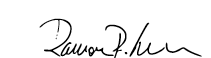
\includegraphics[width=65mm]{figs/logo/assinatura-ramon.png} \\[-4mm]
  \rule[2mm]{70mm}{0.1mm} \\
  \ramon \\[1mm]
  Coordenador do Projeto \\
}

%---------------------------------------------------------------------
\fim